\subsection{The Squad Overlay} 
\label{sec:squad_overlay}

At the root of \name is predictive routing.
%By sharing information among themselves, a user's devices (her \emph{squad}) can model her behavior.
Our goal here is that each online device predicts the probability that it stays online in the near future.
This probability will later be used to create Probabilistic Onion Routes (POR).
A device's connection depends on the activity of its user; thus, a user's devices (her \emph{squad}) want to predict her future behavior.

In this section, we only take interest in one user (called Alice) and her squad.

% Each of Alice's (and Bob's) devices will keep track of its own online and 
% offline behavior.
% They will use a protocol like Sprinkler~\cite{luxey:hal-01704172} to learn about 
% each other's online--offline behavior.
% \commentDaniel{Is that correct?}
% This allows Alice's device swarm to infer a behavioral model for the device 
% swarm and do internal scheduling based on the probability of being online.


\subsubsection{Sharing the user's behavior} % (fold)
\label{sub:sharing_knowledge}

Online devices want to know whether they are likely to stay online in the near future.
Taken separately, each device only knows local information: when Alice used it, and maybe mobility information if it is mobile.
When combining these informations, though, we obtain a sequence of the user's behavior that is far more complete.
For instance, the probability that Alice uses her home computer and workstation simultaneously is null: these devices are too far apart.

The Squad Overlay leverages on a probabilistic dissemination protocol, \textsc{Sprinkler}~\cite{luxey:hal-01704172}, that does just that: 
it allows one's devices to inform one another every time the user performs an action.
Previous work in our team~\cite{luxey:cascade} showed that \textsc{Sprinkler} is resilient to devices churn: 
devices let each other know of what they have missed while offline.
We thus employ \textsc{Sprinkler} to disseminate the user's activity to its squad.

% Each device initially only knows when it is connected, which is not sufficient to make reliable predictions on whether it is likely to stay online.
% If they knew the other devices' connection and disconnection times, they 
% To make a model of the user's behavior, they need to know the whole observation sequence $O$: which device is online at each time step.
% To do so, they employ a probabilistic dissemination protocol, 
% \textsc{Sprinkler}~\cite{luxey:hal-01704172}.
% This allows devices to gossip any new connection information to random peers in 
% the local swarm, ensuring that all devices know the full observation sequence 
% with a very high probability.
% \textsc{Sprinkler} has shown resilient to device churn~\cite{luxey:cascade}, and 
% is thus perfectly suited for our purpose, where a user's devices often 
% disconnect and reconnect. 

% subsection sharing_knowledge (end)

% \subsubsection{Other uses of the Squad Overlay} % (fold)
% \label{ssub:other_uses_of_the_squad_overlay}

\paragraph*{Other uses of the Squad Overlay} In addition to user's behavior, devices use th Squad Overlay for several purposes. Firstly, they share files location: when Alice wants to share a file $f$ that resides on her home computer, using her smartphone as the exchange initiator, her smartphone knows where $f$ is located and can create the route accordingly. 
Secondly, each device is also informed of its user's ongoing file transfers (which serves the next purpose).

\name knows two message types (as will be covered in~\ref{sec:file_exchange}): file chunk, and acknowledgment.
Alice typically wants to receive a file on one particular device; respectively, only one of her devices is interested in acknowledging reception of the file chunks it is sending.
However, \name allows all squad members to receive messages destined to Alice.
Thus, the third complementary purpose of the Squad Overlay is to relay messages among the squad: when a message is not destined to the device that received it, the receiver forwards the message to its final destination.

\subsubsection{Modeling the user's behavior}
\label{sub:a_model_of_the_user_s_behavior}

We need a probabilistic model of the user's behavior to predict its future activity.
In \name, the only data we collect are the connection times of each device.
In this section only, we discretize time. 
We store the connection times in an ever-increasing \emph{sequence} $O=O_1, ..., O_i, ...$ of actions performed at every \emph{round}, that lasts a short period of time $T$. 
$d \in O_t$ thus means that the device $d$ was online from time $t$ to time $t+T$.
Our goal is to predict $O_{t+1}$ knowing $O_t$.

To this end, we model the user's behavior as a Hidden Markov Models (HMMs) of order one, with multiple discrete \emph{observable} processes (one per device) stored in $O$. 
The hidden process $S=S_1, ..., S_i, ...$ represents the user's locations, constituted of a set of $N$ potential locations (e.g. home, work or outside), $N$ being a user-defined parameter.




% In \name, we take interest in users that own several devices, and wish to privately exchange files with each other without revealing .
% To the best of our knowledge, no real-world traces of multi-devices usage over several days exist, as would be needed for the experimental evaluation of our system.
% For that reason, we propose a user behavioral model having the following features:

% \begin{itemize}
% 	\item Each user owns a variable amount of devices. We consider the following device types: mobile, portable, fixed, and server;
% 	\item The user travels between three ``locations'' according to a simple probabilistic model: her home, her workplace, and outside;
% 	\item She makes a different use of her devices depending on her location: at home, she will her laptop that at work; she cannot use her workstation at home.
% \end{itemize}

% To this end, we use a Hidden Markov Model (HMM) of order one, with multiple discrete observation processes. 
% The hidden Markovian process $S$ represents the user's locations, while the \emph{observable} process $O=O_1, \dots, \O_T$ represents the connection state of her devices (either connected or disconnected at any point in time).

% Such a statistical model is simplistic (e.g. it does not encapsulate date \& time nor location), but it is on purpose: simplicity is bliss.
% Given the lack of real-world data for our testbed, building a more complex and realistic user model would add no value to our proposal: 
% our goal is to see devices exhibiting frequent disconnections and reconnections (also called \emph{churn}).
% Our simple model being able to put extravagant stress on our system, it is sufficient to access \name's resilience.

\paragraph*{Formal definition} 

\begin{figure}[t]
\centering
\vspace{-1em}

$$A =
\kbordermatrix{
      & W            & O            & H            \cr
    W & \sfrac{2}{3} & \sfrac{1}{3} & 0            \cr
    O & \sfrac{1}{3} & \sfrac{1}{3} & \sfrac{1}{3} \cr
    H & 0            & \sfrac{1}{3} & \sfrac{2}{3} \\[0.3em]
}, \;
B = 
\kbordermatrix{
      & W     & O   & H   \cr
    o_p & 0.7 & 0.6 & 0.8 \cr
    o_w & 0.7 & 0   & 0   \cr
    o_h & 0   & 0   & 0.7 \cr
    o_l & 0.2 & 0.4 & 0.6 \\[0.3em]
}$$

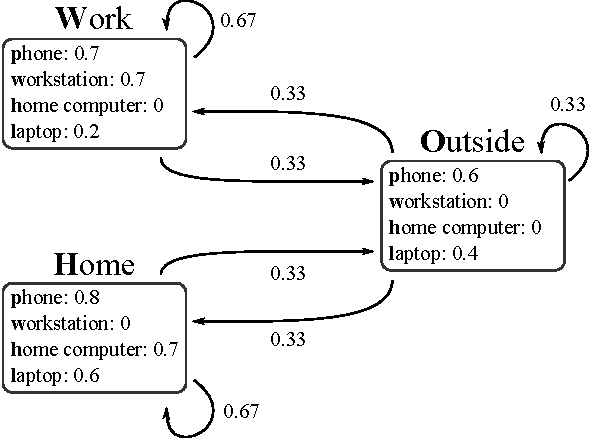
\includegraphics[width=0.9\columnwidth]{figures/hmm.pdf}
\caption{ \label{fig:hmm} Example Hidden Markov Model (HMM) of a user's behavior.}
\end{figure}

We consider a single user, owning a set of $\mathcal{D}$ devices.
Time is discretized \commentAL{Discretized/synchronous time needs more explanation}. Needs, and the devices' observations are independent: Alice can have her laptop and phone connected at the same time.
The hidden process $S=S_1,\dots,S_T$ is built from an alphabet of states $\mathcal{S}$, while the observable process $O=O_1, \dots, \O_T$ contains events from the alphabet $\mathcal{O}$. We define a multivariate HMM $\lambda_N$ as follows:

$$\text{HMM}:\;\lambda_N=(\Pi, A, B)$$

where 
\begin{itemize}
	\item $N$ is the number of states in the system:
	$N = \left| \mathcal{S} \right|$;

	\item $\Pi=\left\{ \pi_i\right\}_{i\in\mathcal{S}}$ is the initial state distribution:\\
	$\pi_i=P[S_1=i]$;

	\item $A = \left\{ a_{i\,j}\right\}_{(i,j)\in\mathcal{S}^2}$ is the state transition matrix:\\
	$a_{i\,j}=P[S_t=j \mid S_{t-1}=i]$;

	\item $B = \left\{ b_{i\,k}\right\}_{(i,k)\in\mathcal{S}\times\mathcal{O}}$ is the matrix of event emission probabilities for each state:
	$b_{i\,k} = P[ k \in O_t \mid S_t = i]$.
\end{itemize}

In our case, the states are the different locations where the user is susceptible to go;
we considered the three following ones: $\mathcal{S}=\left\{ \mathit{work}, \mathit{outside}, \mathit{home} \right\}$. 
There is one event per device $d$: $\mathcal{O} = \left\{ o_d \right\}_{d\in \mathcal{D}}$. Several devices can be connected at the same time, such that $O_t$ is a set, and $o_d \in O_t$ means that device $d$ was connected at time $t$. Devices' connection probabilities are independent.

In \cref{fig:hmm}, we show an example HMM of a user's behavioral HMM, along with its graphical representation (the initial state distribution $\Pi$ was left out for simplicity). 
The represented user possesses a phone and a laptop, that she carries around with her, a home computer, that is only accessible from her home, and a workstation, located at her workplace. She never forgets to turn off her fixed appliances before leaving.

\begin{figure}[t]
\centering
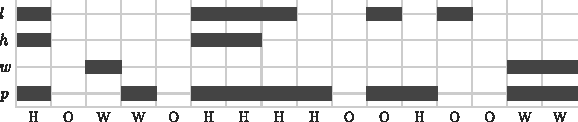
\includegraphics[width=\columnwidth]{figures/sample_usage.pdf}

\caption{\label{fig:sample_usage}Sample device usages using the previous HMM specifications. 
%The bottom line reads the HMM's states: \textbf{W}ork, \textbf{O}utside, and \textbf{H}ome, while the dark lines read when the devices (\textbf{h}ome computer, \textbf{p}hone, and \textbf{w}orkstation) are online.
}

\end{figure}

% Using the toggle events, we compute the device's \emph{connection} events, represented by the multivariate Bernoulli process $C=\left\{ c^{(d)} \right\}_{d\in\mathcal{D}}$. 
% $c^{(d)}_t=1$ (resp. 0) means that the device $d$ was online (resp. offline) at time step $t$.

% We state that every device starts offline, and compute $c^{(d)}_t$ as follows:

% $$ \forall d \in \mathcal{D},
% \begin{cases}
% c^{(d)}_t=0 &\text{when } t=0; \\
% c^{(d)}_t=c^{(d)}_{t-1} \oplus o^{(d)}_t &\text{when } t>0.
% \end{cases}$$

Figure~\ref{fig:sample_usage}, shows a possible trace of the user's behavior, using the parameters depicted in figure~\ref{fig:hmm}. 
It reads the timeline of $o_{d}$ for each device $d$. On the bottom of the graph, the first letter of the user's location is shown at each time step.
We see that devices connections depend on the user's location, and that any number of devices can be connected at the same time.

% Each device starts offline; then, the user either toggles one device per round or does nothing.
% In this figure, we show the device \emph{usage}, that is a consequence of the $\mathit{toggle}$ events defined by the HMM.
% As a consequence, several devices can be online at the same time, as happens in the figure.

% subsubsection formal_definition (end)


\subsubsection{Predicting future behavior} % (fold)
\label{ssub:predicting_future_behavior}
Devices want to predict whether they are likely to be connected in the near future.
This information will be publicly available, and will allow routes selection for the  files exchange between users.

Because devices connections only depend on the users location, we can predict the devices connections in $i$ round $O_{t+i}$ given only the model $\lambda_N$ and the current user's location $S_t$. We first compute the probability that a device $d$ will be connected next turn:

$$
P\left[ o_d \in O_{t} \mid S_{t-1} = s \right] = 
\sum\limits_{s' \in \mathcal{S}} 
a_{s\,s'} * b_{s'\,o_d}.
$$

It is the sum of the probabilities, for each state $s$, that the user switches to $s$ and uses her device.
\commentAL{Following maybe not needed if we only use $t+1$:}
Recursively, predicting $i$ turns in advance follows the same logic:

\begin{multline*}
P\left[ o_d \in O_{t+i} \mid S_{t} = s \right] = \\
\sum\limits_{s' \in \mathcal{S}}
P\left[ S_{t+1} = s' \mid S_t = s \right] * 
P\left[ o_d \in O_{t+i} \mid S_{t+1} = s'\right].
\end{multline*}


\commentAL{In conclusion: we want more unicorns at the Olympic Games.}

\commentAL{I don't mention prediction yet since I am not sure we get good enough results.}